\documentclass[11pt,a4paper]{article}
\usepackage[utf8]{inputenc}
\usepackage{amsmath}
\usepackage{amsfonts}
\usepackage{amssymb}
\usepackage{graphicx}
\usepackage{url}
\usepackage{pinlabel}

%% Uncomment zero or one of the following three sections

%\usepackage{newtxtext}
%\usepackage[libertine,bigdelims,vvarbb]{newtxmath}
%\usepackage[cal=boondoxo]{mathalfa}

%\usepackage{newpxtext,eulerpx}

%\usepackage[cmintegrals,cmbraces]{newtxmath}
%\usepackage{ebgaramond-maths}




\author{Oleg Soloviev}
\title{Simple example of labelling with pinlabel}
\begin{document}
	
	\maketitle
	
	Please note how the same font is used for the text and for the labels inside the diagram. 
	
	Try to comment/uncomment font selection in the preamble.

	
	\begin{equation}\label{eq1}
	i^{(k)}=x^{(k)}\mathcal{P}(i/x^{(k)})
	\end{equation}
	
	\begin{figure}[htb]
		\labellist
		\small\hair 2pt
		\pinlabel {$i$} [l] at 234 637
		\pinlabel {$x^{(k)}$} [l] at 263 676
		\pinlabel {$i^{(k)}=x^{(k)}\mathcal{P}(i/x^{(k)})$} [l] at 229 704
		\endlabellist
		\centering
		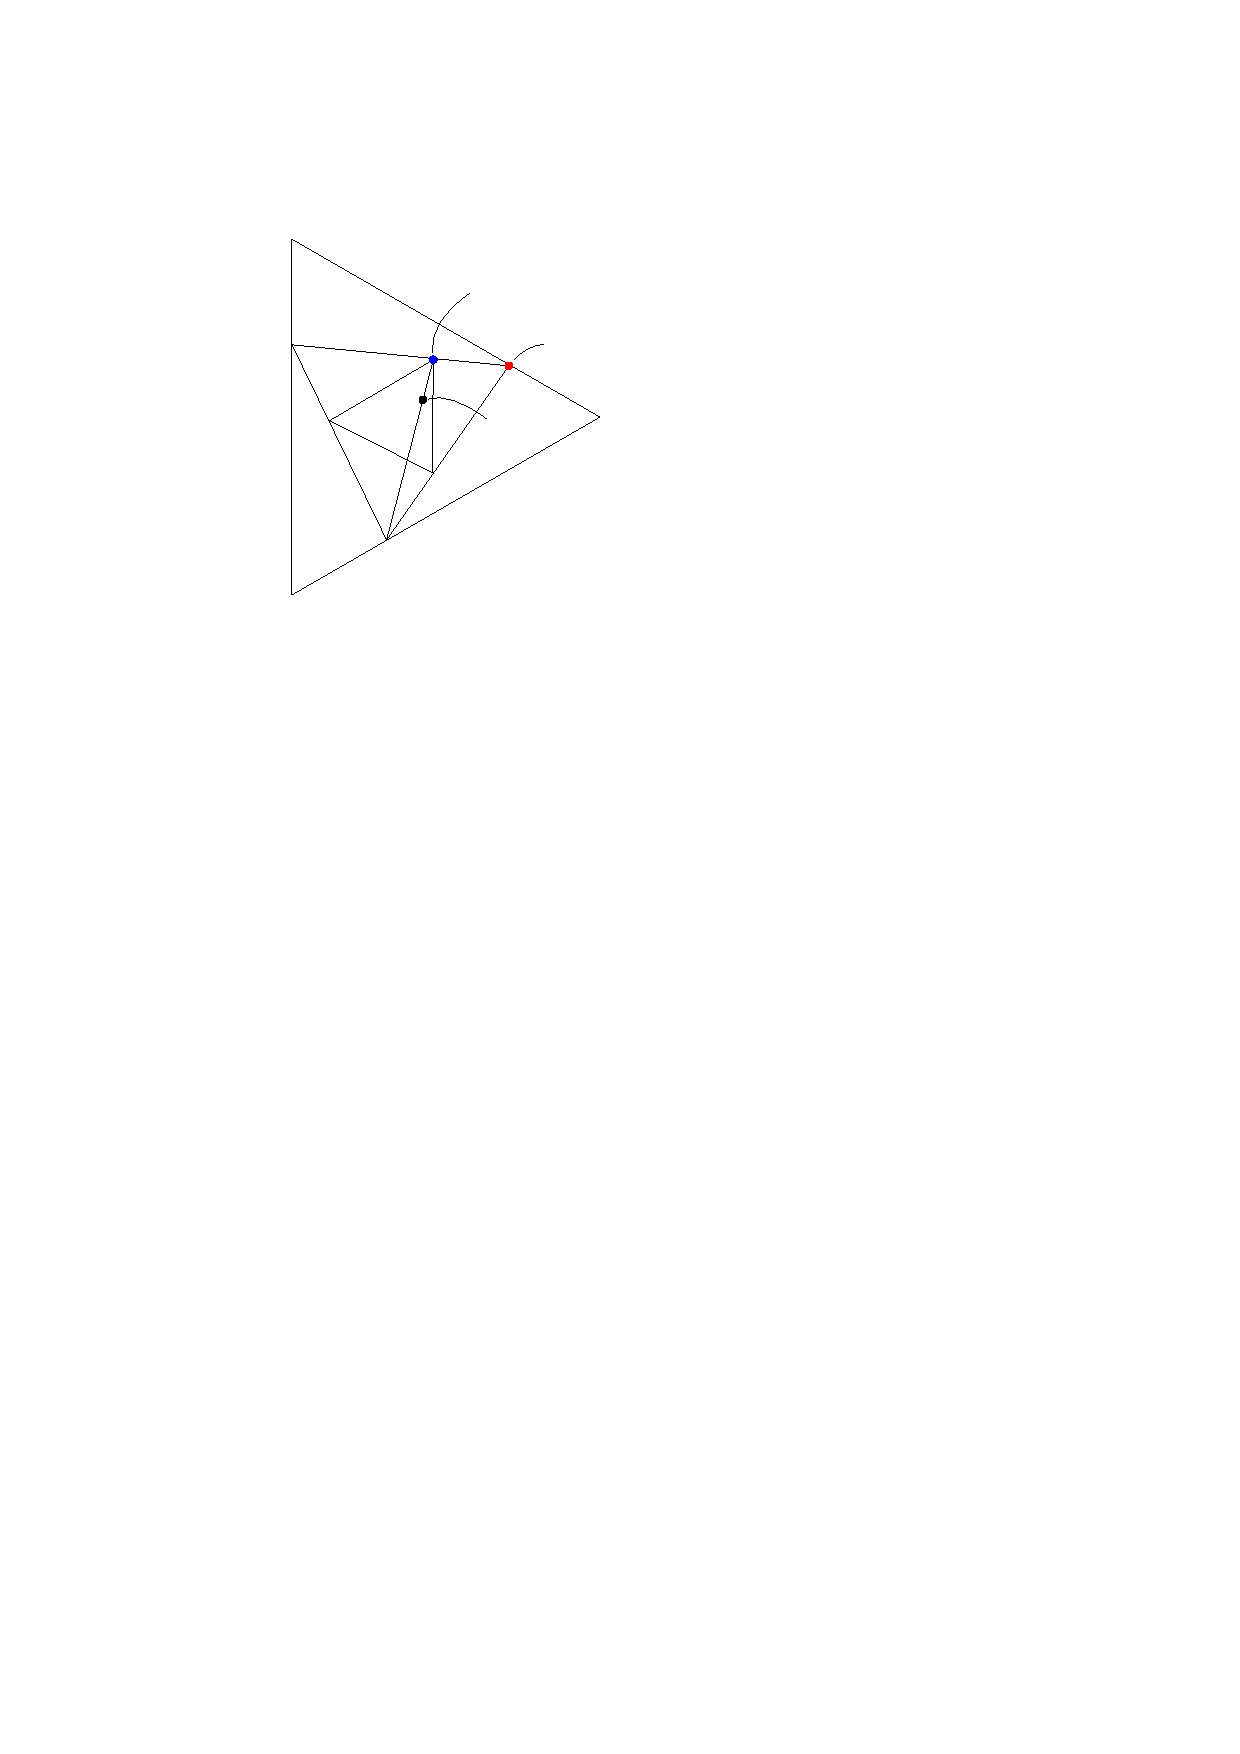
\includegraphics[scale=1.0]{simplex}
		\caption{
			Take $i^{(k)}$ as projection of $i$ on the  side of simplex formed by $x{(k)}$ to get $i^{(k)}$.  $x^{(k+1)}$ is then defined from equation~\eqref{eq1}.
		}
		\label{fig:label}
	\end{figure}



	
	Please see the package documentation\footnote{Type \texttt{texdoc pinlabel} in command line} for all advanced options.
\end{document}